\documentclass[aps,jcp,preprint,superscriptaddress]{revtex4}

\usepackage[utf8]{inputenc}
\usepackage{amsmath, amssymb}
\usepackage{tabularx,booktabs,array,dcolumn}
\usepackage{setspace}
\usepackage{vmargin}
\usepackage{graphicx,psfrag,subfigure}
\usepackage{color}
\usepackage[all]{xy}

\usepackage{enumitem}
\usepackage{mdframed}
\usepackage{xcolor}

\sloppy \frenchspacing \clubpenalty=10000 \widowpenalty=10000

\begin{document}

\title{
Melting point convergence with various potentials, effect of the number of atoms, walkers and steps}


\author{}
\affiliation{}
\email{}

\date{\today}

\maketitle

%%%%%%%%%%%%%%%%%%%%%%%%%%%%%%%%%%%%%%%%%%%%%%%%%%%%%%%%%%%%%%%%%%%%%%%%%%
%
% Introduction
%
%%%%%%%%%%%%%%%%%%%%%%%%%%%%%%%%%%%%%%%%%%%%%%%%%%%%%%%%%%%%%%%%%%%%%%%%%%
\section{mW model of water}
\begin{figure}[hbt]
\begin{center}
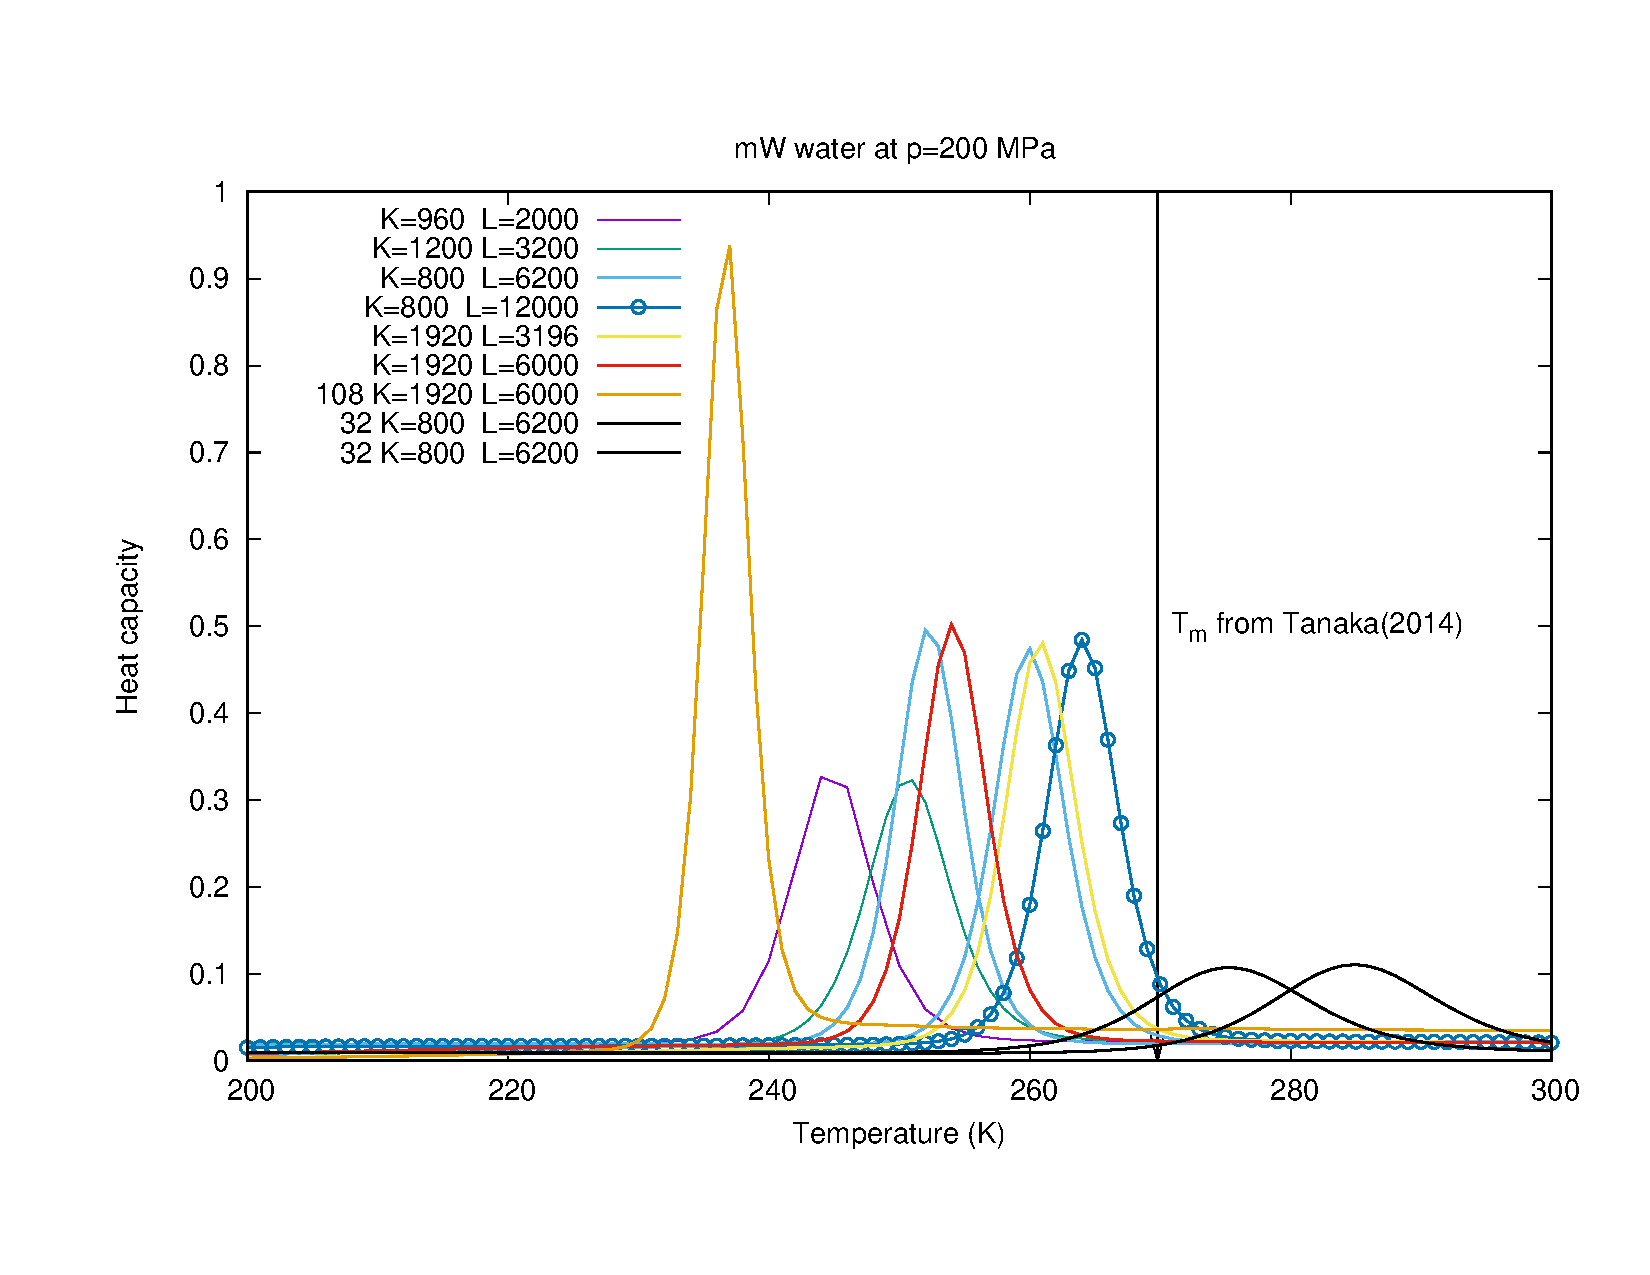
\includegraphics[width=14cm]{mW-fig.pdf}
\end{center}
\vspace{-20pt}
\caption {Predicted melting temperature of the mW model at 200 MPa, for 32, 64 and 128 atoms.}
\label{fig:mW}
\end{figure}


\end{document}
